\newpage
\chapter{Messungen}
\section{Messsystem}
Blabla Bla verschiedene Messsysteme für die unterschiedlichen Aufgaben.\\
unteranderem  StarLab für die elektromagnetische Feldmessungen von strahlenden Körpern.\\

BlaBla Netzwerkanalysator zum bestimmen der Streuparameter
\subsection{StarLab}
Das Messsystem  StarLab der \textit{mvG microwave vision Gruppe} ermöglicht das Messen von Antennen und strahlenden Körpern. Es ist ein Messsystem für Hochfrequenzsysteme, die im Mikrowellenbereich strahlen. Das System misst Antennen im Zylinder- und Kugelkoordinatensystem. Misst das System das elektromagnetische Feld eines Körpers im Zylinderkoordinatensystem, so wird ein Testobjekt auf einem motorisierten Schlitten durch die Mitte des StarLab gezogen. Dabei zeichnen die 12 im Kreis angeordneten Kreuzantennen das abgestrahlte elektromagnetische Feld auf. 
Wird das von einem Testobjekt abgestrahlte elektromagnetische Feld im Kugelkoordinatensystem aufgenommen, wird das Testobjekt genau im Zentrum der Messapparatur platziert. Der Drehteller, auf dem sich das Testobjekt befindet, dreht sich während eines Messzyklus um 360 Grad. 
Das StarLab Messsystem besteht aus  zwei Teilen. Der erste Teil ist die Messapparatur. Diese beinhaltet zwölf kreuzförmige im Kreis angeordnete Antennen welche im orangen Kreis um das Messobjekt angebracht sind.  Die Antennen sind alle ins Zentrum gerichtet und zwischen ihnen liegen je 22.5 Grad. Das gibt eine Abdeckung von 270 Grad. In Zentrum des Messsystems ist eine Testplattform. Diese ist von einem Schrittmotor angetrieben. Dies ermöglicht, dass das elektromagnetische Feld eines Testobjekts aus allen Richtungen aufgezeichnet werden kann. Der Frequenzgenerator des StarLab hat einen Signalfrequenzbereich von 650 MHz bis 6 GHz. Ein Testobjekt darf maximal einen Durchmesser von 45 cm aufweisen.
Die Absorberkegel sind neben dem orangen Messring befestigt. Diese Kegel verhindern Reflektionen der elektromagnetischen Wellen. Da ansonsten nicht nur die primäre Abstrahlung des Testobjekts, sondern ein Gemisch aus Abstrahlung und Reflexionen aufgezeichnet wird. Aus demselben Grunde können die beiden Öffnungen der Messapparatur mit Absorberpanels verschlossen werden. Die Abbildung xx zeigt ein Messobjekt im Zentrum der Messapparatur. 

Das Messobjekt wird mit Polystyrol angehoben, damit das Testobjekt genau in der Mitte der Messapparatur platziert wird. Polystyrol hat nur minimalen Einfluss auf die elektromagnetischen Wellen und ist daher gut geeignet um Objekte zu stützen. Ein weiterer Vorteil des Polystyrols ist das geringe Gewicht von $1.05 g/cm^3$. Die maximale Last, bestehend aus Drehteller und Testobjekt, darf  10 kg  nicht überschreiten. Zudem besitzt das Polystyrol eine sehr tiefe Dielektrizitätskonstante. Sie beträgt $\varepsilon_r=1.03$ bei 50 Hz. Zum Vergleich, das als ideal betrachtete Vakuum  besitzt ein $\varepsilon_r=1$ bei 50Hz. Der Verlustwinkel bei 1 MHz ist sehr klein mit $0.05*10^-3$.
\cite{StarLab,Polystyrol_Datenblatt,WikiPermitt} 
%Quelle: https://de.wikipedia.org/wiki/Permittivität
%Quelle: http://www.kern.de


\subsection{Netzwerkanalysator}
Ein Netzwerkanalysator wird in der Elektronik, der Nachrichtentechnik und besonders in der Hochfrequenztechnik eingesetzt. Seine Aufgaben umfassen das Aufnehmen der Streuparameter (S-Parameter), also Reflexion und Transmission von elektrischen Signalwellen an
Messobjekten. Der Netzwerkanalysator zeichnet die S Parameter als Funktion der Frequenz auf. Der Netzwerkanalysator sendet ein Signal, die  hinlaufende Welle genannt, zum  Messobjekt. Das Messobjekt wird in der englischen Literatur  \textit{DUT} ein device under test genannt. Die  Frequenz, Amplitude und Phase der hinlaufenden Welle sind bekannt. Das Messobjekt reflektiert einen Teil der hinlaufenden Welle. Dieser Teil wird weglaufende Welle genannt. Sie wird ohne in das Testobjekt einzudringen, am Eingang des Messobjekts, zum Netzwerkanalysator zurück reflektiert. Der Rest läuft in das Messobjekt, wird dort verändert, das heisst gedämpft, verstärkt oder phasenverschoben. Der transmittierte Signalanteil tritt am Ausgang des DUT als übertragenes Signal in Erscheinung. Die durch das DUT veränderte und am Ausgang anliegende Signalwelle wird auch  weglaufende Welle genannt.

Aus dem Verhältnis von reflektiertem zu gesendetem Signal wird die Reflexion des Messobjektes gemessen. Der $S_{11}$ Wert gibt in dB die Rückflussdämpfung an. Diese wird in enlischer der Literatur \textit{Return Loss} genannt.
Der $S_{21}$ Wert gibt Auskunft über das Verhältnis des übertragenen Signal zu dem gesendeten Signal. Dabei wird die  Transmission des Messobjektes gemessen. 
Die Abbildung \ref{NetzwerkanalysatorZweiTor} zeigt diesen Zusammenhang auf.
\cite{NetzwerkanalyzorTUDarmstadt}
%%%%%%%%%%%%%%%%%%%%%%%%%%%%%%%%%%%
\begin{figure}[!ht]
\begin{center}
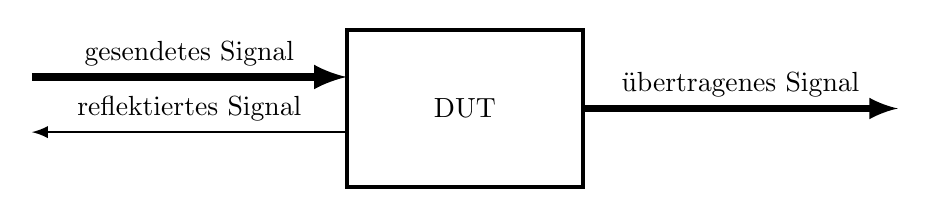
\begin{tikzpicture}
	\draw[line width=1.5pt](4, 1) rectangle (7, 3) node at (5.5,2) {DUT};
	\draw[line width=3pt, ->, >=latex](0, 2.4) -- (4, 2.4) node at (2,2.7) {gesendetes Signal};
	\draw[line width=2.5pt, ->, >=latex](7, 2) -- (11, 2) node at (9,2.3) {übertragenes Signal};
	\draw[line width=1pt, ->, >=latex](4, 1.7) -- (0, 1.7) node at (2,2) {reflektiertes Signal};
	%\draw[line width=1.5pt](3, 0) rectangle (5, 1);
\end{tikzpicture}
\end{center}
	\caption{Ermittlung der S-Parameter am Zweitor}
	\label{NetzwerkanalysatorZweiTor}
\end{figure}
%%%%%%%%%%%%%%%%%%%%%%%%%%%%%%%%
%%%%%%%%%%%%%%%%%%%%%%%%%%%%%%%%%%%
\begin{figure}[!ht]
\begin{center}
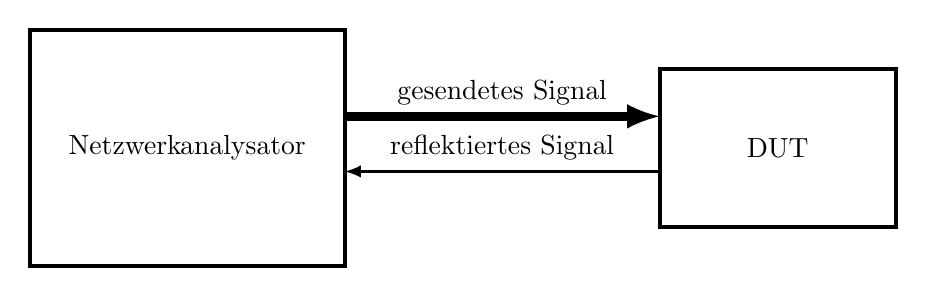
\begin{tikzpicture}
	\draw[line width=1.5pt](0, 0.5) rectangle (4, 3.5) node at (2,2) {Netzwerkanalysator};
	\draw[line width=1.5pt](8, 1) rectangle (11, 3) node at (9.5,2) {DUT};
	\draw[line width=3pt, ->, >=latex](4, 2.4) -- (8, 2.4) node at (6,2.7) {gesendetes Signal};
	\draw[line width=1pt, ->, >=latex](8, 1.7) -- (4, 1.7) node at (6,2) {reflektiertes Signal};
	%\draw[line width=1.5pt](3, 0) rectangle (5, 1);
\end{tikzpicture}
\end{center}
	\caption{Ermittlung der $S_{11}$ Parameter am Zweitor}
	\label{NetzwerkanalysatorS11}
\end{figure}
%%%%%%%%%%%%%%%%%%%%%%%%%%%%%%%%
%%%%%%%%%%%%%%%%%%%%%%%%%%%%%%%%%%%
\begin{figure}[!ht]
\begin{center}
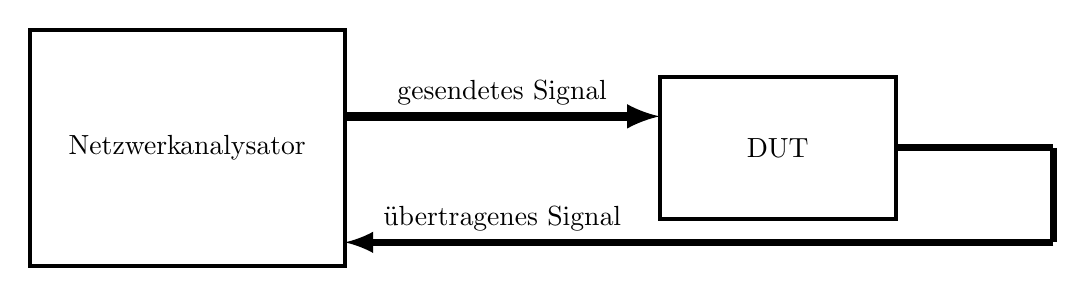
\begin{tikzpicture}
	\draw[line width=1.5pt](0, 1.5) rectangle (4, 4.5) node at (2,3) {Netzwerkanalysator};
	\draw[line width=1.5pt](8, 2.1) rectangle (11, 3.9) node at (9.5,3) {DUT};
	\draw[line width=3pt, ->, >=latex](4, 3.4) -- (8, 3.4) node at (6,3.7) {gesendetes Signal};
	\draw[line width=2.5pt, ->, >=latex](13, 1.8) -- (4, 1.8) node at (6,2.1) {übertragenes Signal};
	\draw[line width=2.5pt] (11, 3) -- (13, 3);
	\draw[line width=2.5pt] (13, 3) -- (13, 1.8);
\end{tikzpicture}
\end{center}
	\caption{Ermittlung der $S_{21}$ Parameter am Zweitor}
	\label{NetzwerkanalysatorS21}
\end{figure}
%%%%%%%%%%%%%%%%%%%%%%%%%%%%%%%%
\newpage
\section{Mess Setup}
Um zukünftig die Kommunikation der "Connect 1" Geräte mit einem Smartphone zu ermöglichen wird ein neues Antennenkonzept für das "Bluetooth Low Eneergie Network" gesucht. Aus der Konzeptphase ist herausgeganen,dass das Abstrahlverhalten von Dipolantennen genauer untersucht wird und mit Simulationen ein optimales Antennedesign für den Einsatz in den "Connect 1" Geräten gesucht wird. Die drei Design mit dem grösten Wirkungsgrad $\eta_{rad}$ werden in einen Testserie geprüft.\\
Die Antennendesigs wurden Anhand der im EMPIRE XPU erstellten Draft-Daten gefertigt. Die Antennenstrukturen sind aus 3M 8111 Kupferband hergestellt. Dieses Band eigent sich sehr gut um die der Testphase ein einfaches Design, kostgünstig und schnell umzusetzen. Die gewünschte Antennenstruktur wird dem Skalpel aus dem Band ausgeschnitten und auf einen Träger aufgeklebt. \\
Da jede Antenne eine Zuleitung braucht, wurden am Fusspunkt der Kupferbandantennen ein \textit{semi rigid Koaxialkabel} angebracht. Da es sich bei einem Dipol um eine symetrische Antenne handelt, muss auch die Zuleitung symetrisch sein. Aus diesem Grund wurde der Innenleiter des Koaxialkabel am Einspeisepunkt des einen Dipolarms und der Mantel des Koaxialkabels mit Einspeisepunkt des zwiten Dipolarm verlötet.\\
Die \textit{semi rigid Koaxialkabel} von $HUBER+SUHNER$ des Typs $SUCOFORM_47_CU$ beistzt eine Impedanz von $50  \pm 2\Omega$. Das Ende des Koaxialkabel ist mit einem SMA Gewinde versehen.\\

\textbf{Testobjekte}
Auf die Impelementierung verwisen
\textbf{Erwartungen}
Auf dei Simulationen verweisen

Alle drei Antennedesigns wurden im EMPIRE XPU designed und simuliert. Sie weissen alle eine Abstrahleffizienz von mehr als $\eta{rad}$ von 60 $\%$ auf. 
\subsubsection{Messergebnisse}
Bla bla\\
Text\\
Tabellen\\
\subsubsection{Fazit der Messung xx}
Vergleich aus der erartungshaltung und den Messresultaten